\chapter{Results and Discussion}
\label{chap:results}

\graphicspath{{figs/results/}}

This chapter provides the performance metrics and resulting visuals of the described methods. \autoref{chap:methodology} describes these methods on a conceptual level, and \autoref{chap:implementation} unveils the implementation details.

First, this chapter describes the measuring methodology and testing environment. Then, it shows the collected results for this application without point cloud rendering acceleration and with acceleration methods applied.


\section{Measuring methodology}

\subsection{Testing environment}

We collected the results from the application running on a computer with the following technical specifications:

\begin{itemize}
    \item CPU: AMD Ryzen 7 3750H @ 2.3GHz, 4 cores (8 threads)
    \item GPU: NVIDIA GeForce GTX 1650
    \item RAM: 16 GB DDR4
\end{itemize}

We used the Unity Editor 2020.2.2f1 to run the developed algorithms.

\subsection{Metrics}

To evaluate the result, we proposed the following metrics:

\begin{itemize}
    \item Framerate (frames per second, FPS) – this metric helps assess the algorithm's performance.
    \item Memory consumption (megabytes, MB) – this metric helps assess the algorithm's resource consumption.
    \item Visual quality (absence of defects, amount of detail saved) – this metric is subjective.
\end{itemize}

\subsection{Testing scenario}

It is crucial to provide the generalized testing scenario to make the testing unbiased. In terms of this work, we tested the single component of the larger software project. The \autoref{chap:introduction} gives a brief description of the major project.

The testing scenario steps are the following:

\begin{enumerate}
    \item Select the algorithm and set the parameters.
    \item Import or re-import\footnote{The asset should be reimported in case it was imported earlier with different parameters.} LAS file with the test point cloud.
    \item Add the imported point cloud to the scene.
    \item Run the scene.
    \item Collect the metrics: the framerate in the Unity Editor, the memory usage in the operating system task manager or another resource monitor, and the rendered scene on the editor screen.
\end{enumerate}


\section{Collected results}

To minimize the environmental impact on application performance results, we made ten measurements for each testing scenario. We collected the following data by averaging ten measures during the testing.


\subsection{Generating LODs}

\subsubsection{Urban environment}

In this scenario, we measured the performance of the LOD generation algorithm on the urban scene that was captured from the part of Bangkok, Thailand [citation here].

\begin{table}[h]
    \centering
    \begin{tabular}{l|l|l|l}
    LODs & FPS & Memory (GB) & Visual quality (relative) \\ \hline
    800, 1600, 3200 & 25.1 & 3.2 & High \\
    400, 800, 1600 & 49.5 & 3.2 & Medium \\
    200, 800, 1600 & 65.3 & 3.2 & Low
    \end{tabular}
    
    \caption{Results for LOD generation algorithm on urban environment.}
    \label{tab:results:lod-urban}
\end{table}

\begin{figure}[htb]
    \centering
    
    \begin{subfigure}{0.45\textwidth}
        \centering
        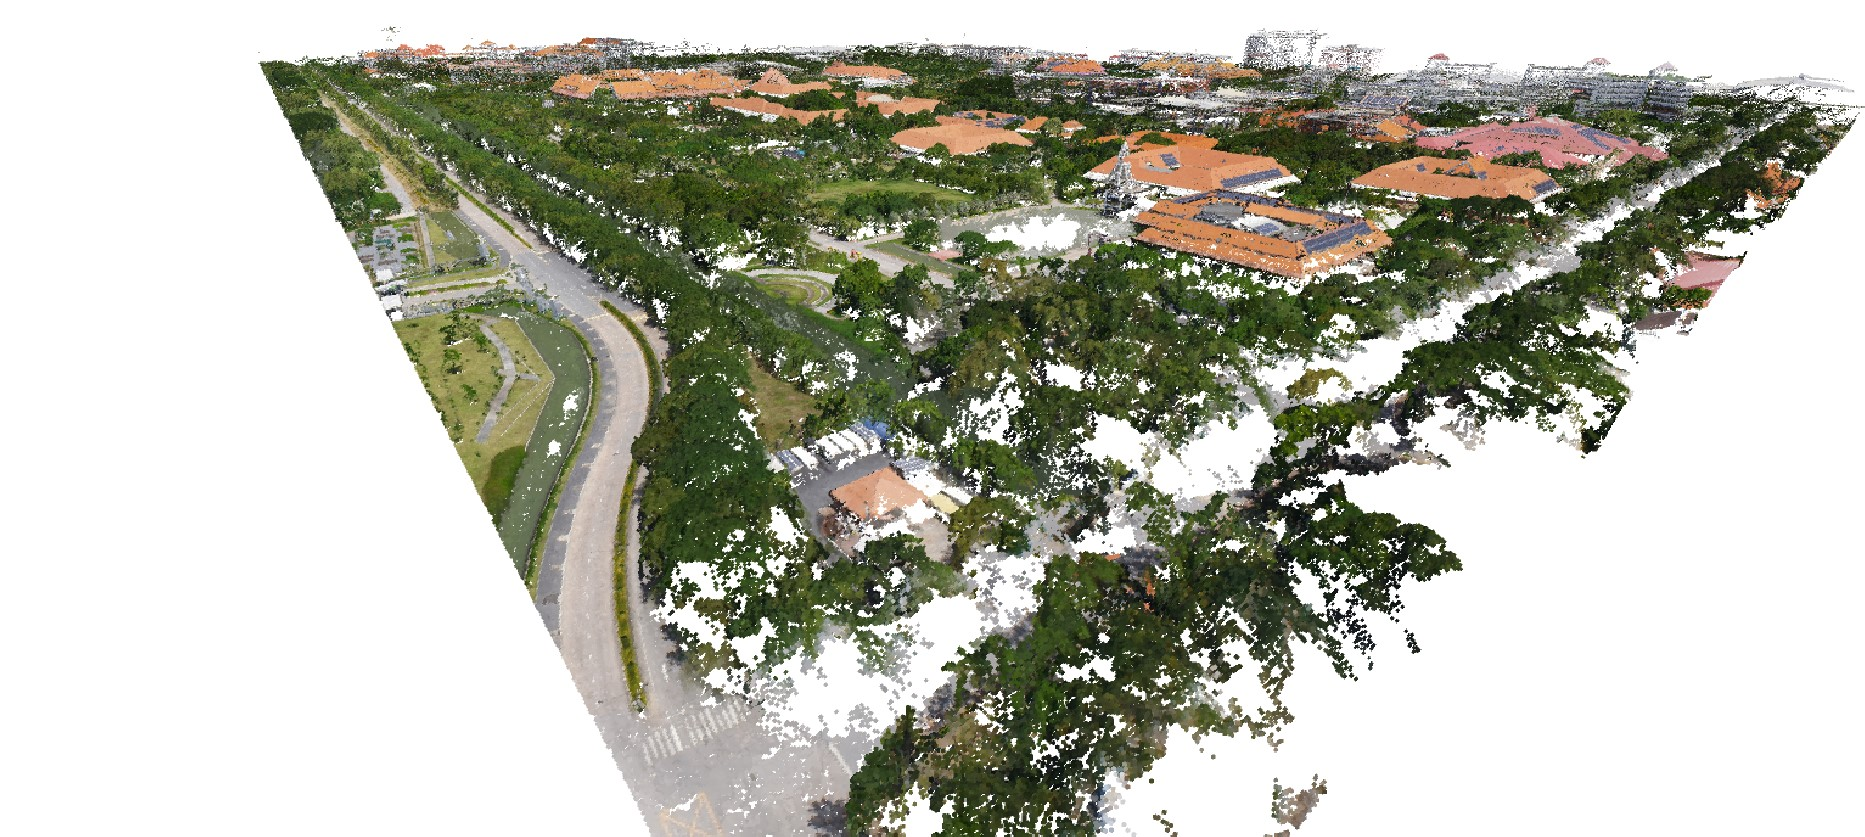
\includegraphics[width=\textwidth]{lod-urban-800.jpg}
        \caption{LOD 800-1600-3200}
        \label{fig:results:lod-urban-800}
    \end{subfigure}
    %
    \begin{subfigure}{0.45\textwidth}
        \centering
        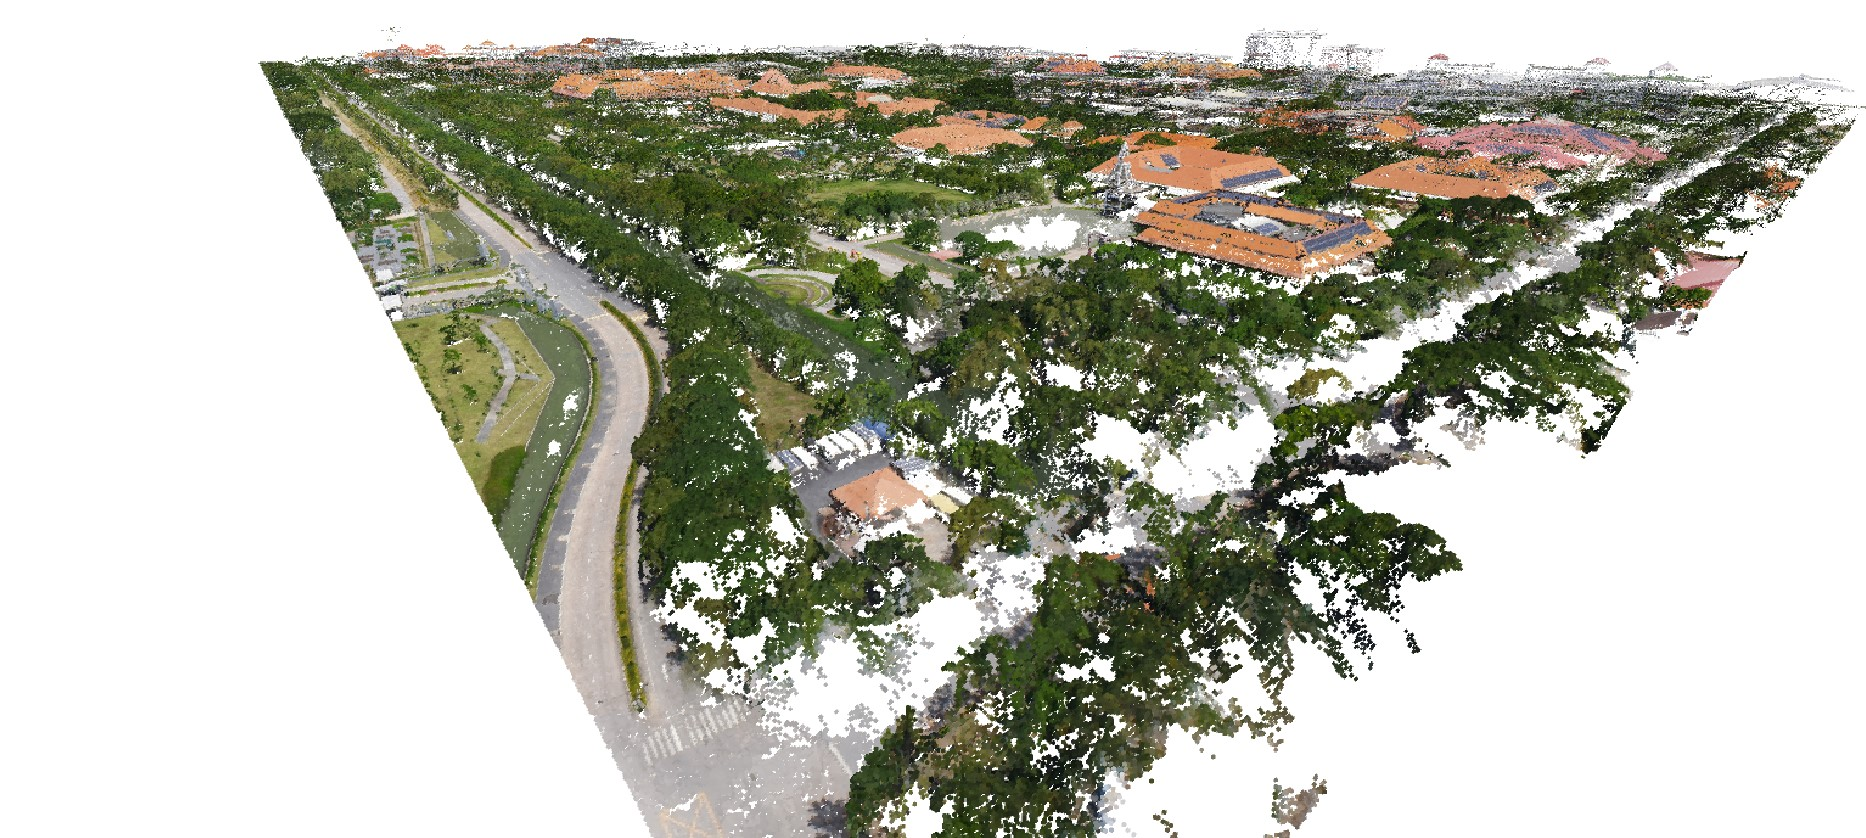
\includegraphics[width=\textwidth]{lod-urban-400.jpg}
        \caption{LOD 400-800-1600}
        \label{fig:results:lod-urban-400}
    \end{subfigure}
    
    \begin{subfigure}{0.45\textwidth}
        \centering
        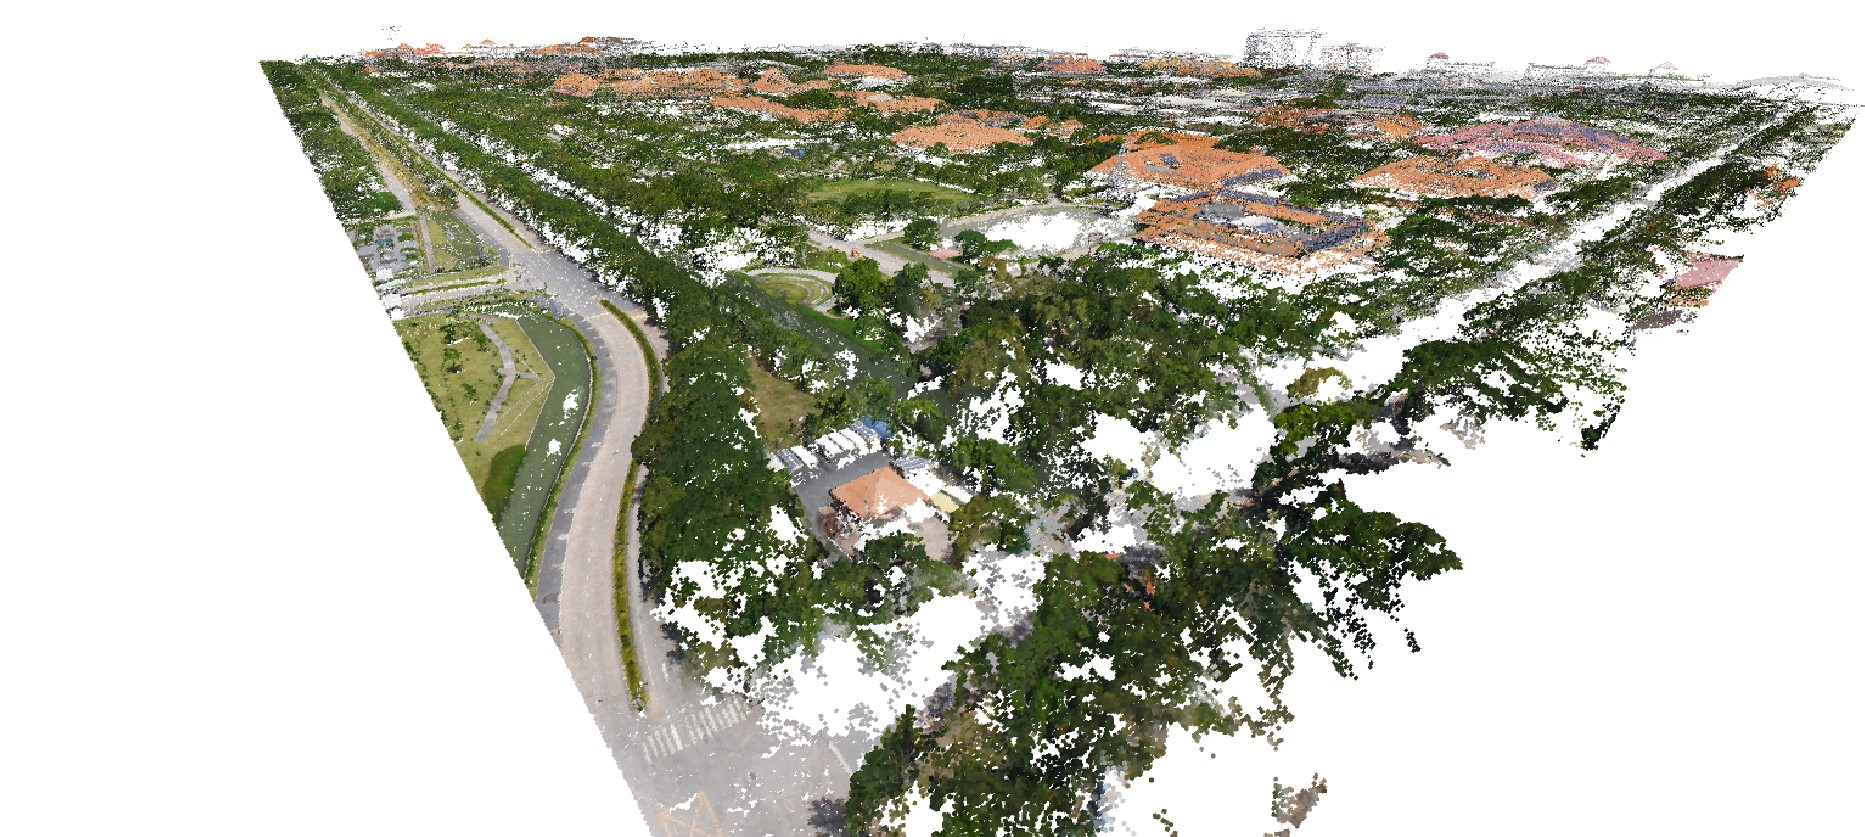
\includegraphics[width=\textwidth]{lod-urban-200.jpg}
        \caption{LOD 200-800-1600}
        \label{fig:results:lod-urban-200}
    \end{subfigure}
    
    \caption{Urban scene rendered with LODs.}
\end{figure}

On the \autoref{fig:results:lod-urban-800} the picture quality is acceptable. This setting saves most of the detail and delivers a high render distance without significant quality loss. However, it is hard to examine the scene in the close distance as the emptiness between points becomes noticeable.

Unlike the previous one, on the \autoref{fig:results:lod-urban-400} this setting delivers a lower render distance, and the algorithm renders far chunks with lower quality.

On the \autoref{fig:results:lod-urban-800} the setting provides the lowest quality for the far chunks.


\subsubsection{Landscape environment}

In this scenario, we measured the performance of the LOD generation algorithm in the countryside scene that was captured nearby the Innopolis, Tatarstan, Russian Federation.

\begin{table}[htb]
    \centering
    \begin{tabular}{l|l|l|l}
    LODs & FPS & Memory (GB) & Visual quality (relative) \\ \hline
    300, 600,   1200 & 17.0 & 2.4 & High \\
    200, 400, 800 & 21.6 & 2.4 & Meduim \\
    100, 200, 400 & 42.2 & 2.4 & Low
    \end{tabular}
    
    \caption{Results for LOD generation algorithm on landscape environment.}
    \label{tab:results:lod-landscape}
\end{table}

\begin{figure}[h]
    \centering
    
    \begin{subfigure}{0.45\textwidth}
        \centering
        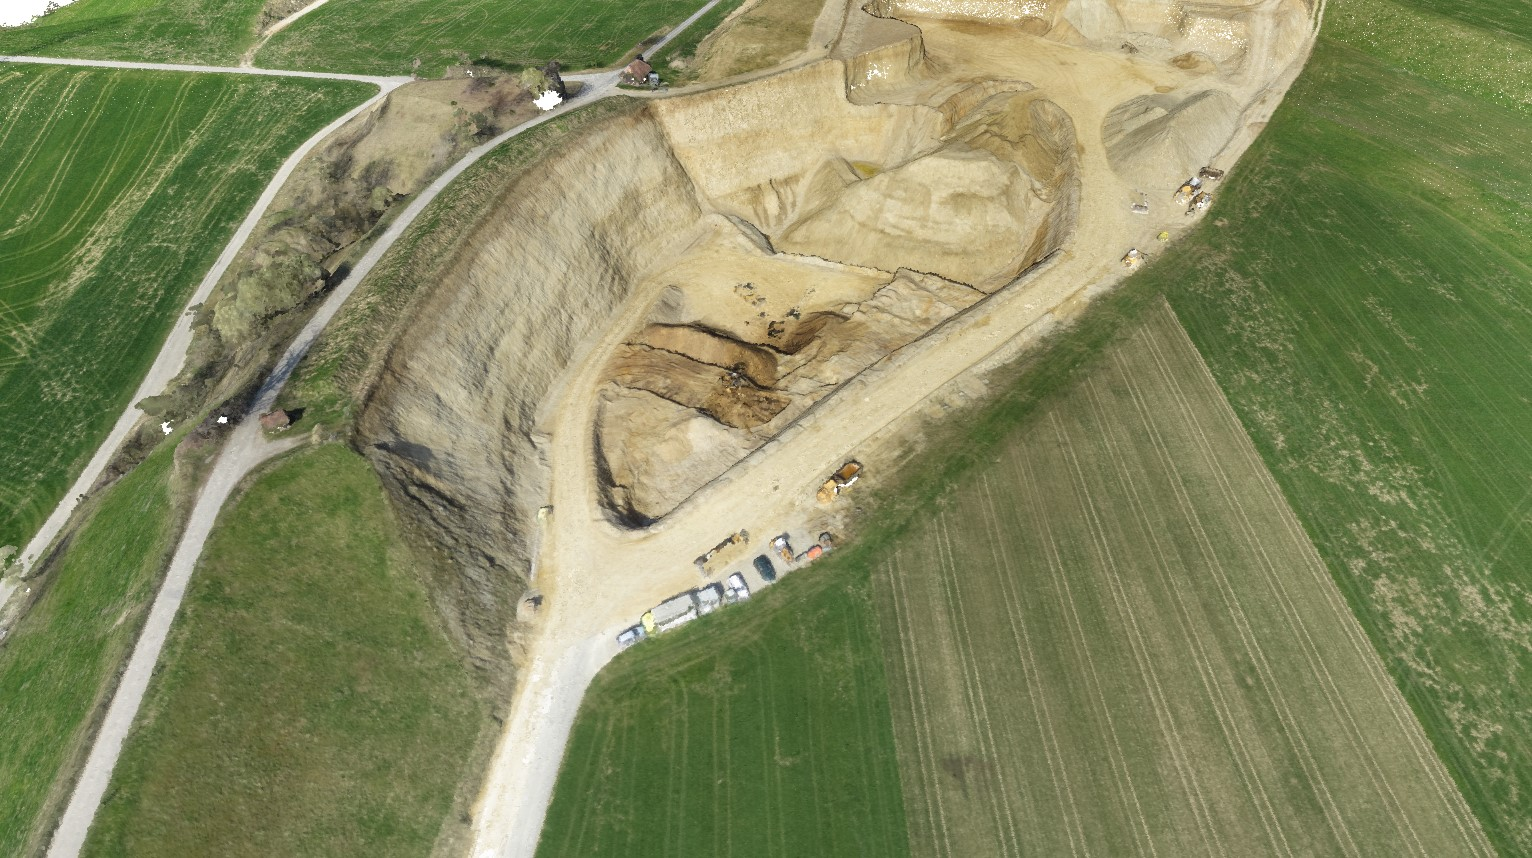
\includegraphics[width=\textwidth]{lod-landscape-300.jpg}
        \caption{LOD 300-600-1200}
        \label{fig:results:lod-landscape-300}
    \end{subfigure}
    %
    \begin{subfigure}{0.45\textwidth}
        \centering
        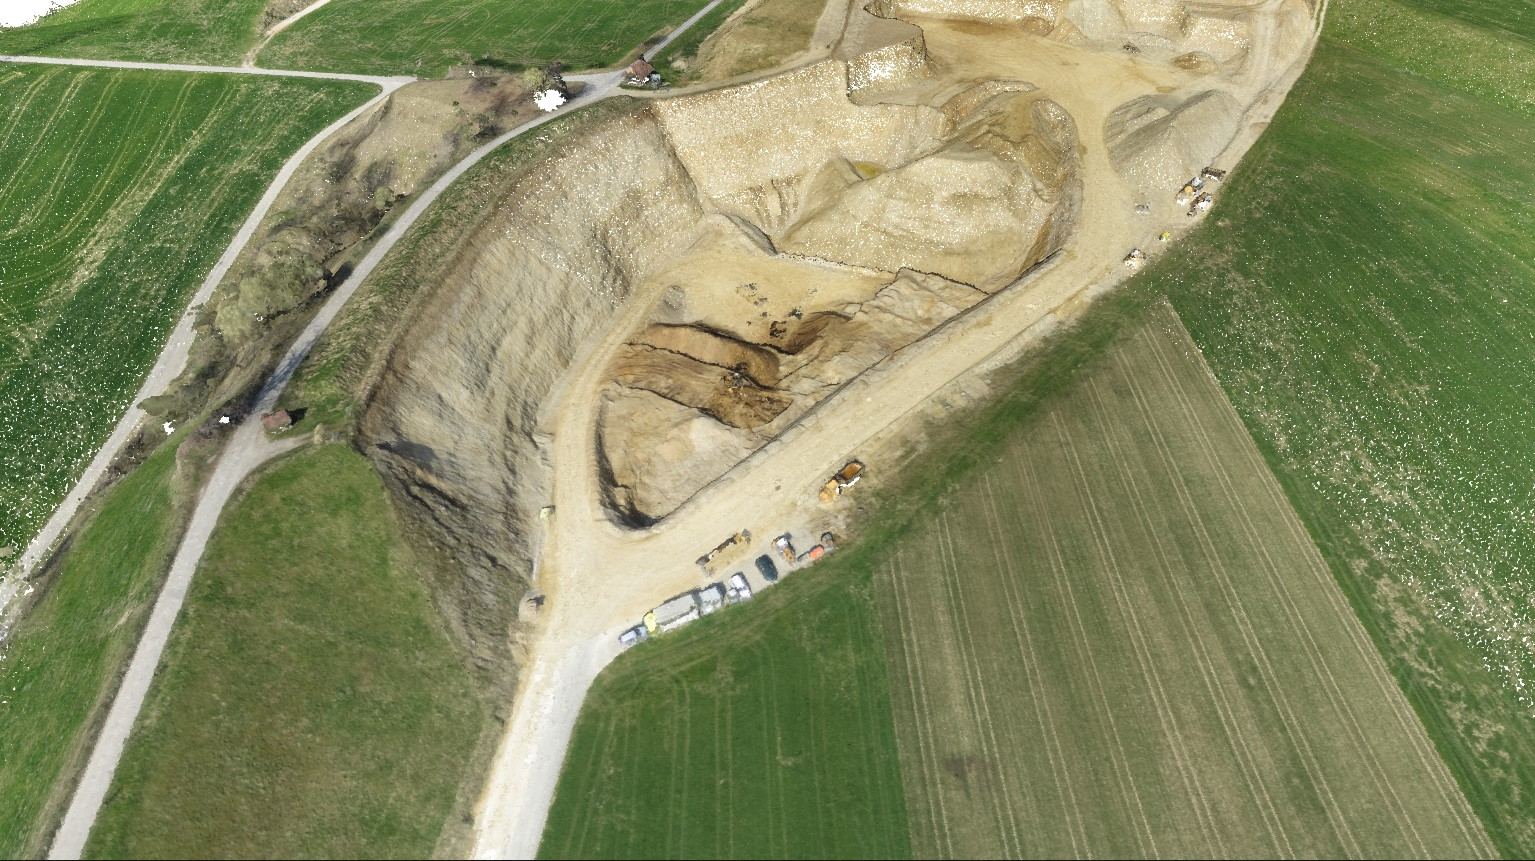
\includegraphics[width=\textwidth]{lod-landscape-200.jpg}
        \caption{LOD 200-400-800}
        \label{fig:results:lod-landscape-200}
    \end{subfigure}
    
    \begin{subfigure}{0.45\textwidth}
        \centering
        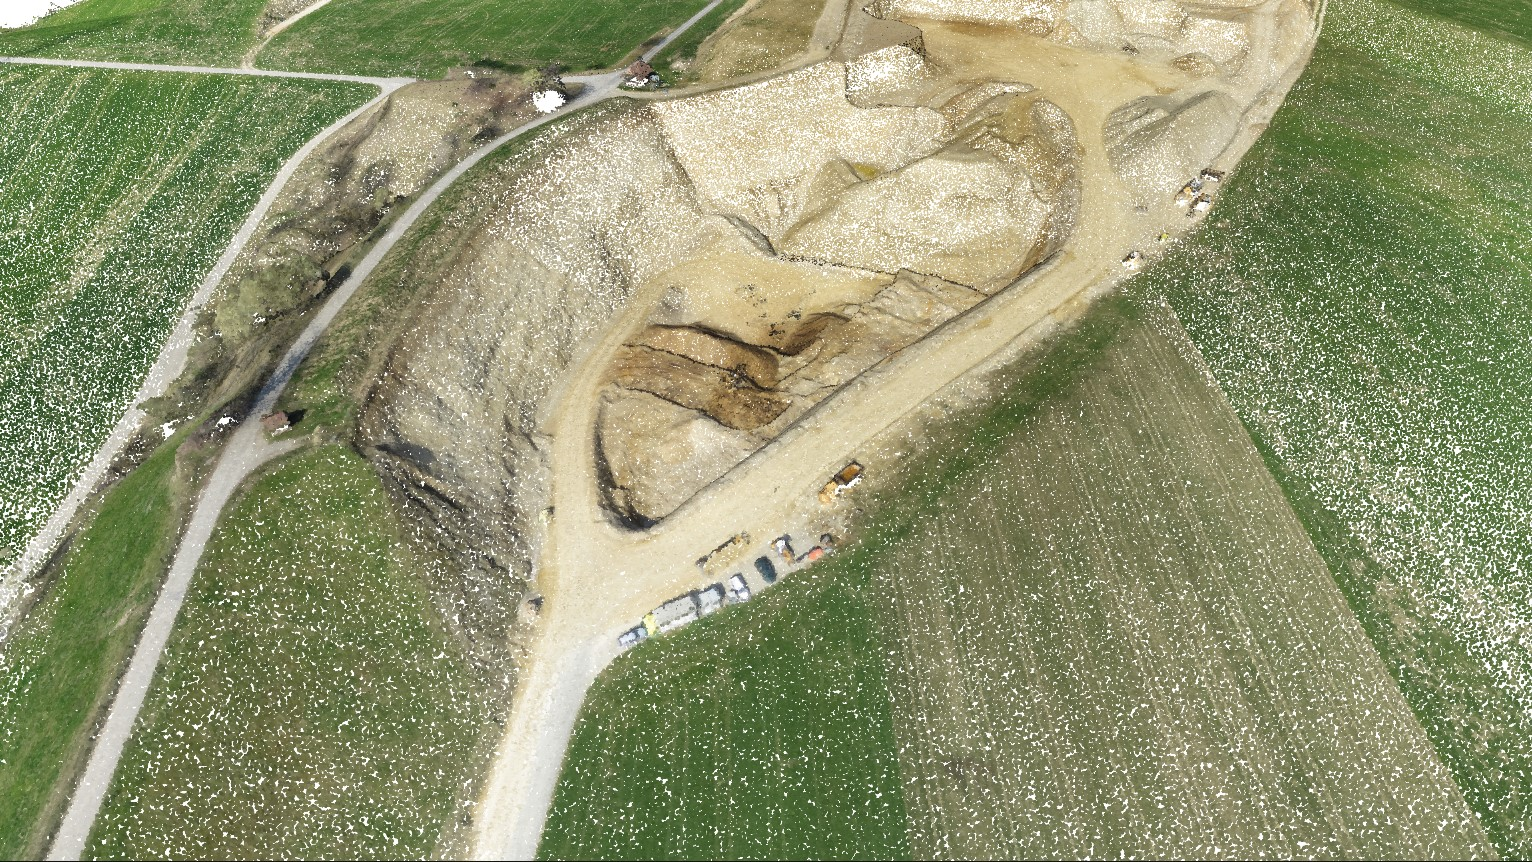
\includegraphics[width=\textwidth]{lod-landscape-100.jpg}
        \caption{LOD 100-200-400}
        \label{fig:results:lod-landscape-100}
    \end{subfigure}
    
    \caption{Landscape scene rendered with LODs.}
\end{figure}

On the \autoref{fig:results:lod-landscape-300} the picture quality is acceptable. However, it is hard to examine the scene in the close distance as the emptiness between points becomes noticeable.

On the \autoref{fig:results:lod-landscape-200} the picture quality is acceptable. However, as fewer points are rendered, a grain appears on the model.

On the \autoref{fig:results:lod-landscape-100} the picture quality is not acceptable. Due to the low number of rendered points, a noticeable grain appeared on the model.


\subsection{Mesh generation}

\subsubsection{Urban environment}

In this scenario, we measured the performance of the mesh creation algorithm on the urban scene that was captured from the part of Bangkok, Thailand [citation here].

\begin{table}[htb]
    \centering
    \begin{tabular}{l|l|l|l}
    Chunk resolution & FPS & Memory (MB) & Visual quality (relative) \\ \hline
    256 & 71.4 & 551.9 & High \\
    128 & 130.4 & 498.6 & Meduim \\
    64 & 182.9 & 446.0 & Low
    \end{tabular}
    
    \caption{Results for Mesh generation algorithm on urban environment.}
    \label{tab:results:mesh-urban}
\end{table}

\begin{figure}[h]
    \centering
    
    \begin{subfigure}{0.45\textwidth}
        \centering
        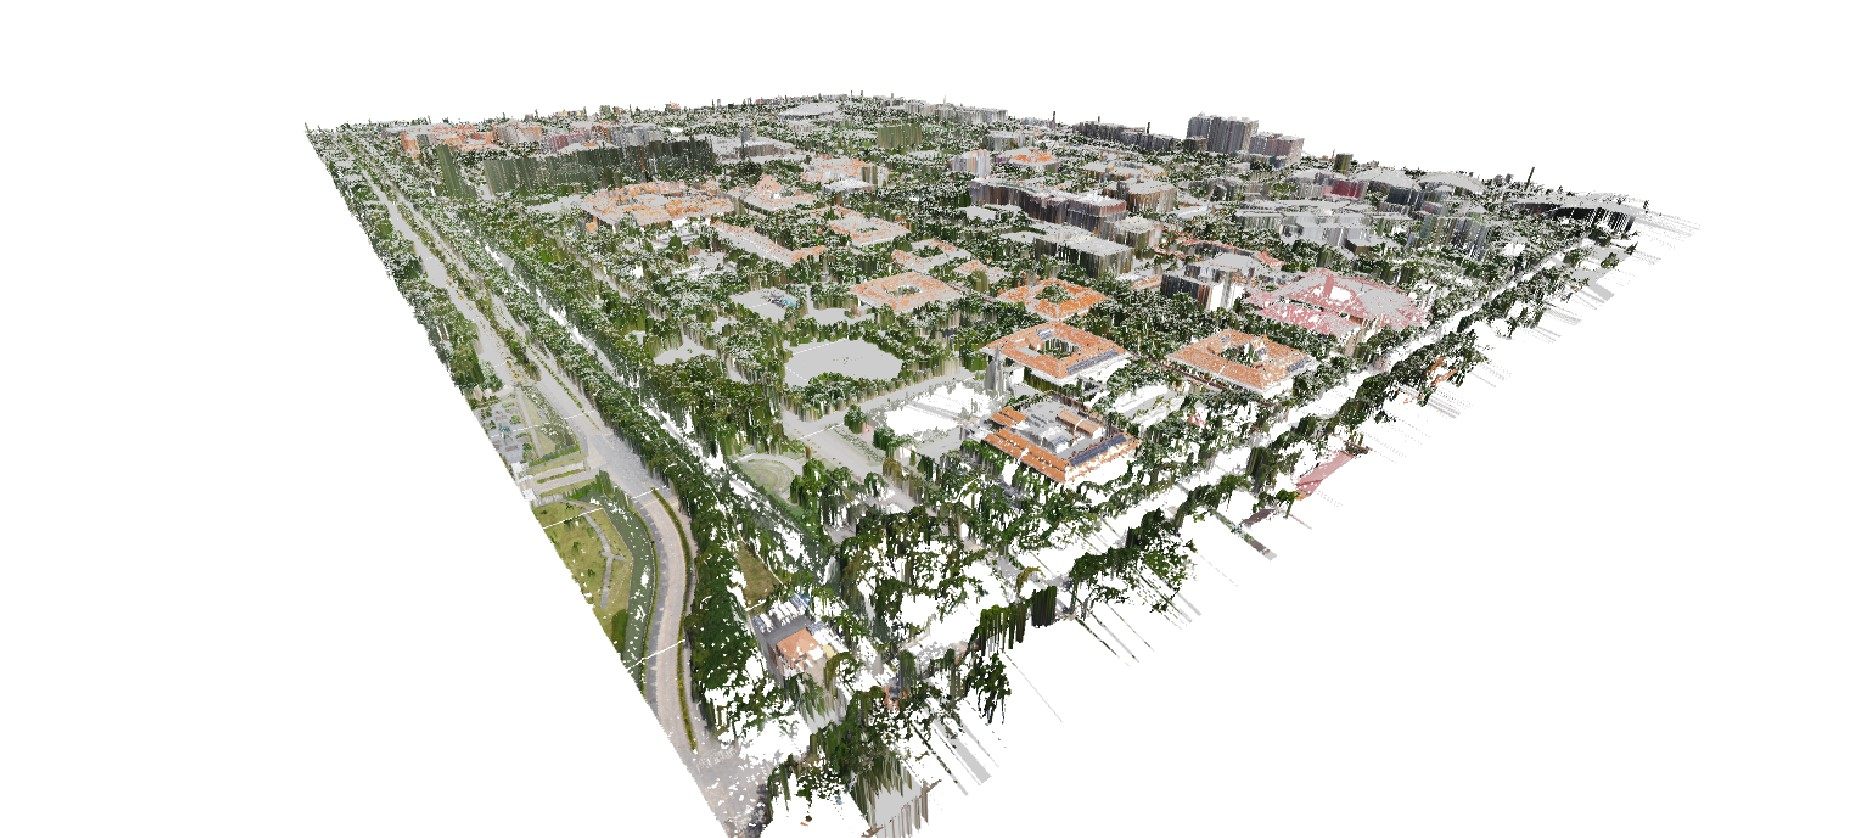
\includegraphics[width=\textwidth]{mesh-urban-256.jpg}
        \caption{Mesh w. chunk resolution 256}
        \label{fig:results:mesh-urban-256}
    \end{subfigure}
    %
    \begin{subfigure}{0.45\textwidth}
        \centering
        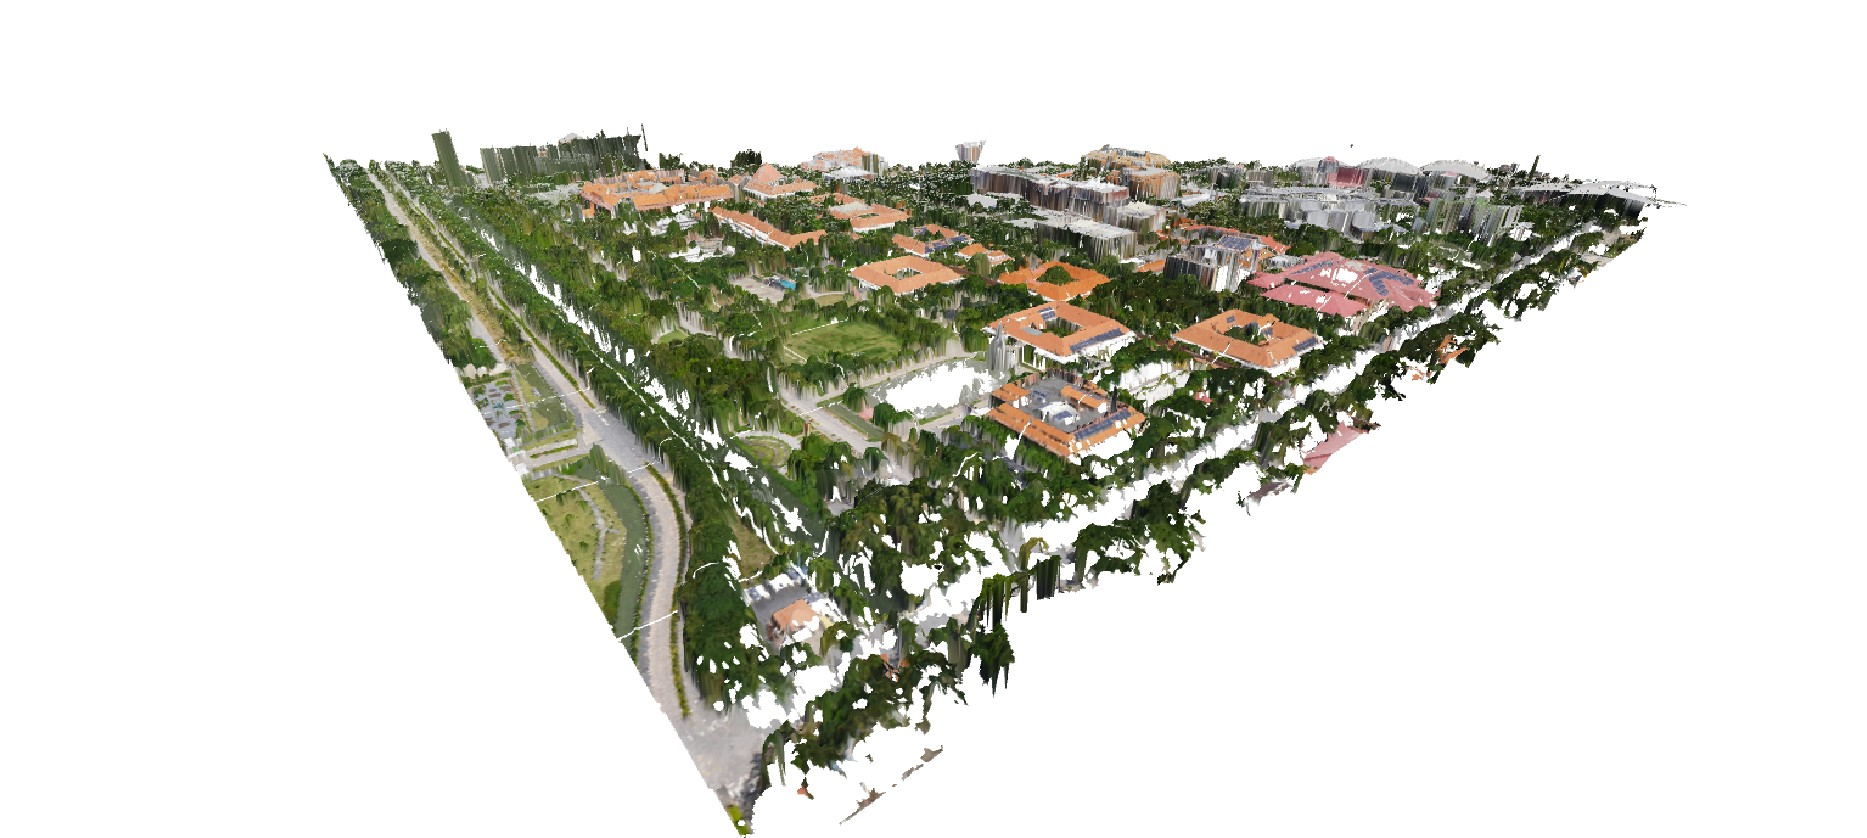
\includegraphics[width=\textwidth]{mesh-urban-128.jpg}
        \caption{Mesh w. chunk resolution 128}
        \label{fig:results:mesh-urban-128}
    \end{subfigure}
    
    \begin{subfigure}{0.45\textwidth}
        \centering
        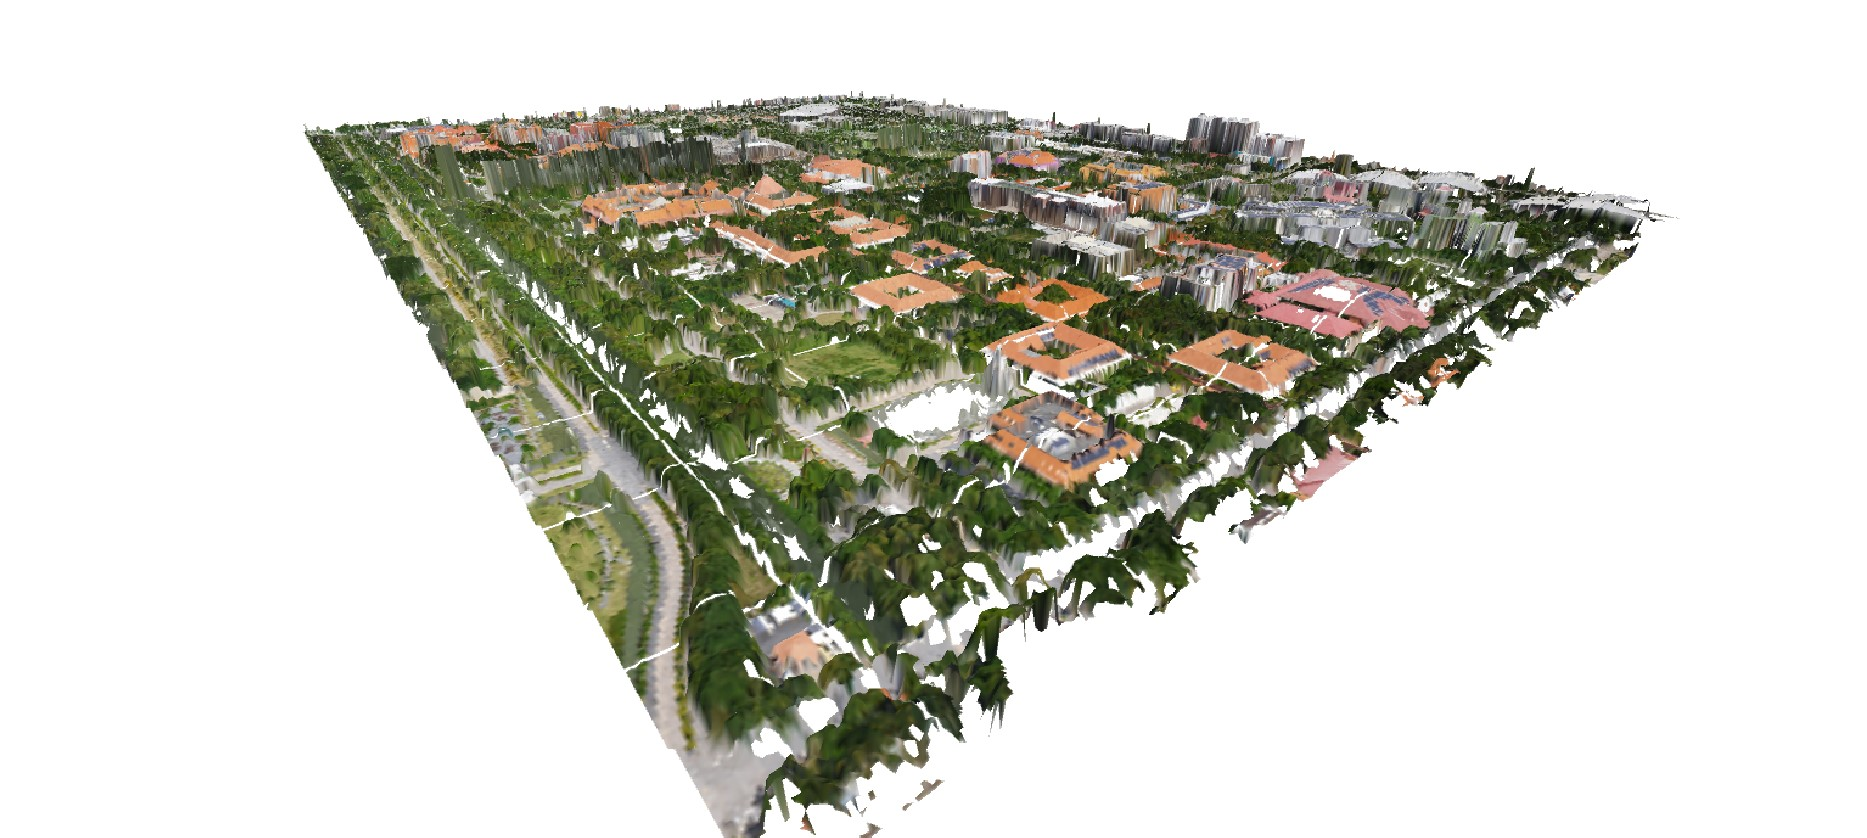
\includegraphics[width=\textwidth]{mesh-urban-64.jpg}
        \caption{Mesh w. chunk resolution 64}
        \label{fig:results:mesh-urban-64}
    \end{subfigure}
    
    \caption{Urban scene rendered with generated mesh.}
\end{figure}

On the \autoref{fig:results:mesh-urban-256} the setting saves the most of detail on the model.

On the \autoref{fig:results:mesh-urban-128} the setting shows less detail than the previous one, but the image has less noise than in the previous setting.

On the \autoref{fig:results:mesh-urban-64} the setting drops most of the detail, and the chunk borders become noticeable.


\subsubsection{Landscape environment}

In this scenario, we measured the performance of the mesh generation algorithm in the countryside scene that was captured nearby the Innopolis, Tatarstan, Russian Federation.

\begin{table}[htb]
    \centering
    \begin{tabular}{l|l|l|l}
    Chunk resolution & FPS & Memory (MB) & Visual quality (relative) \\ \hline
    256 & 148.8 & 453.2 & High \\
    128 & 203.6 & 425.2 & Meduim \\
    64 & 219.3 & 379.7 & Low
    \end{tabular}
    
    \caption{Results for Mesh generation algorithm on urban environment.}
    \label{tab:results:mesh-landscape}
\end{table}

\begin{figure}[h]
    \centering
    
    \begin{subfigure}{0.45\textwidth}
        \centering
        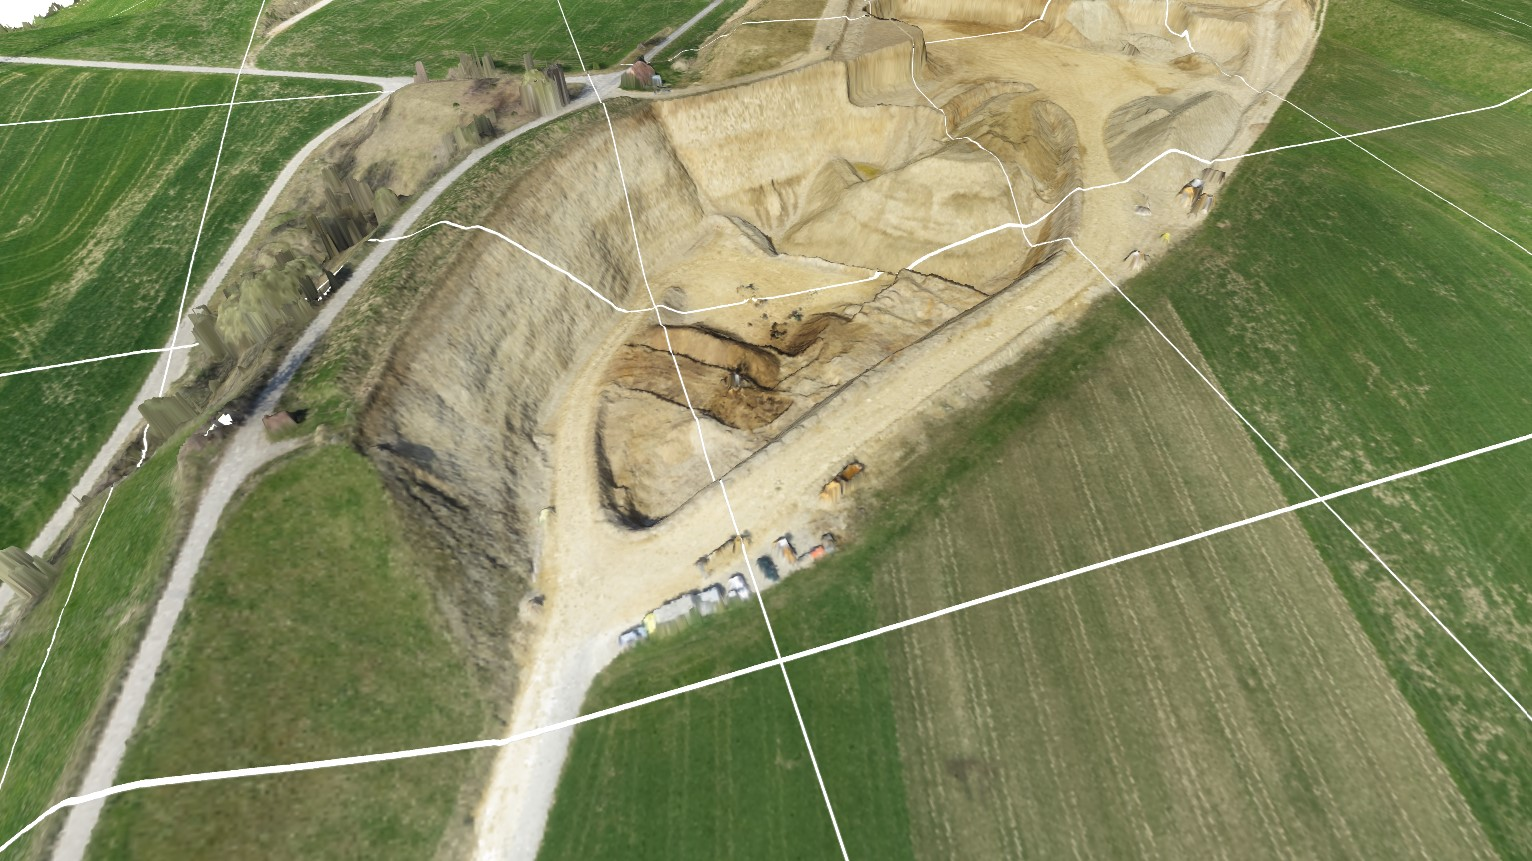
\includegraphics[width=\textwidth]{mesh-landscape-256.jpg}
        \caption{Mesh w. chunk resolution 256}
        \label{fig:results:mesh-landscape-256}
    \end{subfigure}
    %
    \begin{subfigure}{0.45\textwidth}
        \centering
        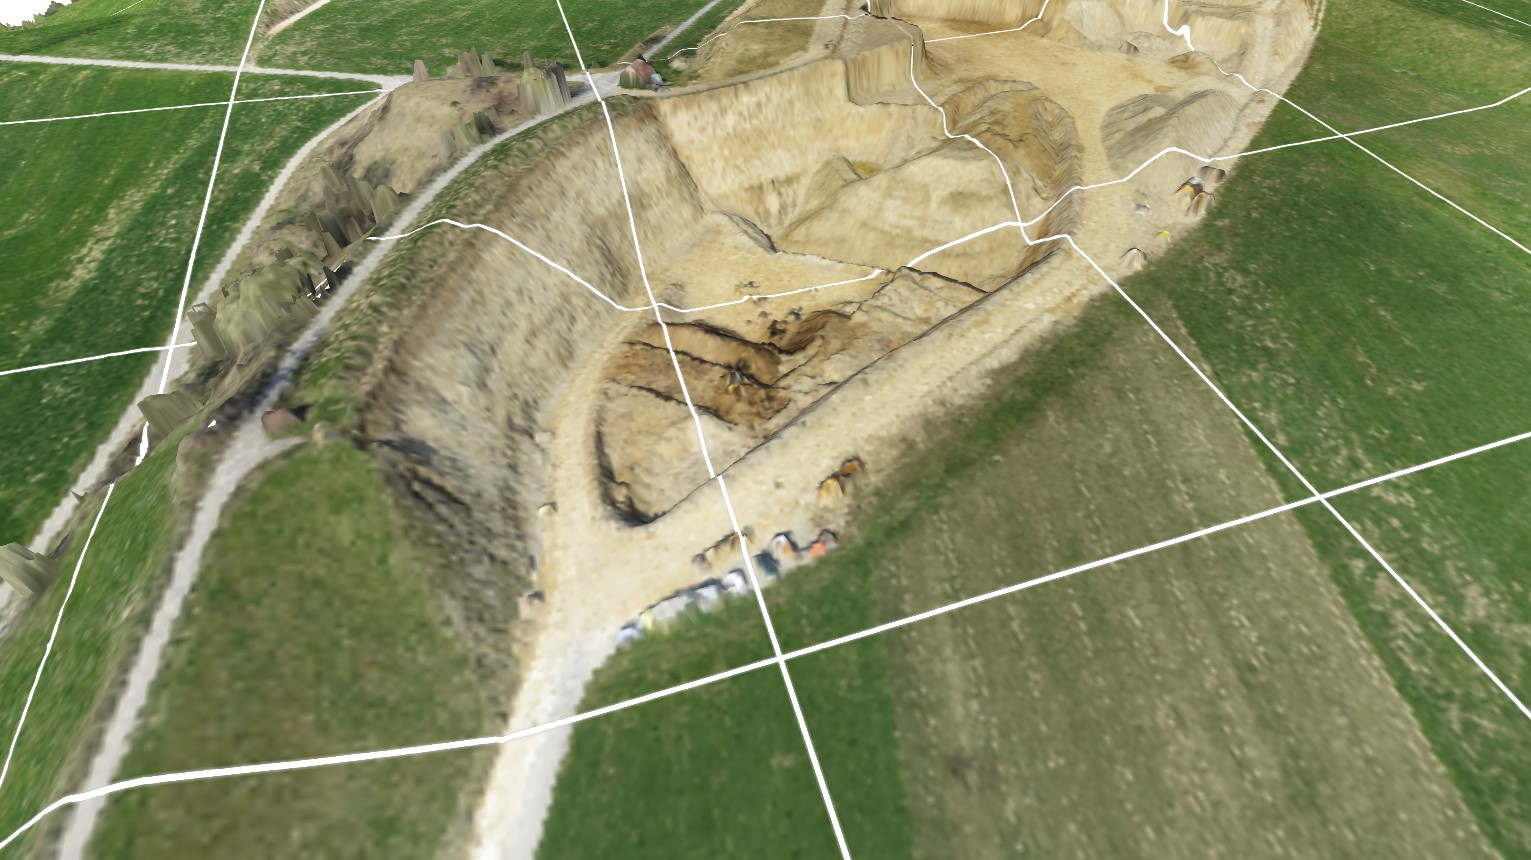
\includegraphics[width=\textwidth]{mesh-landscape-128.jpg}
        \caption{Mesh w. chunk resolution 128}
        \label{fig:results:mesh-landscape-128}
    \end{subfigure}
    
    \begin{subfigure}{0.45\textwidth}
        \centering
        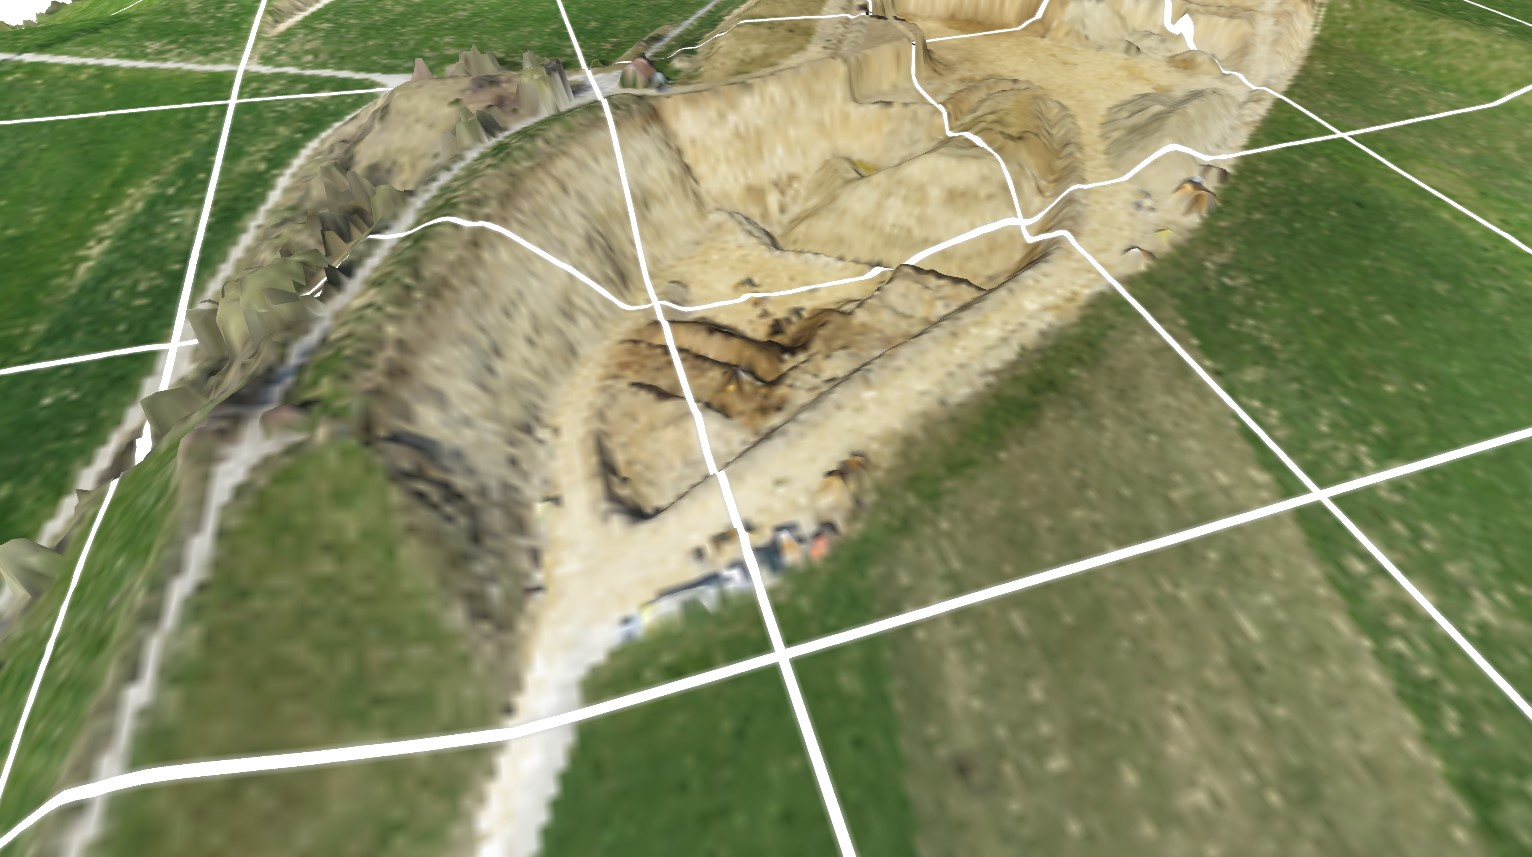
\includegraphics[width=\textwidth]{mesh-landscape-64.jpg}
        \caption{Mesh w. chunk resolution 64}
        \label{fig:results:mesh-landscape-64}
    \end{subfigure}
    
    \caption{Landscape scene rendered with generated mesh.}
\end{figure}

As the scene does not contain much detail, the picture quality is equally good on all samples. However, as the chunk size decreases, the chunk borders become thicker and more noticeable and occur more often.

All rendered visuals are available in a bigger size in \autoref{appex:rendered-scenes}.

\section{Evaluation}

\subsection{Framerate}

The \autoref{fig:results:graph-fps} summarizes the results on framerate.

\begin{figure}[h]
    \centering
    
    \begin{subfigure}{0.3\textwidth}
        \centering
        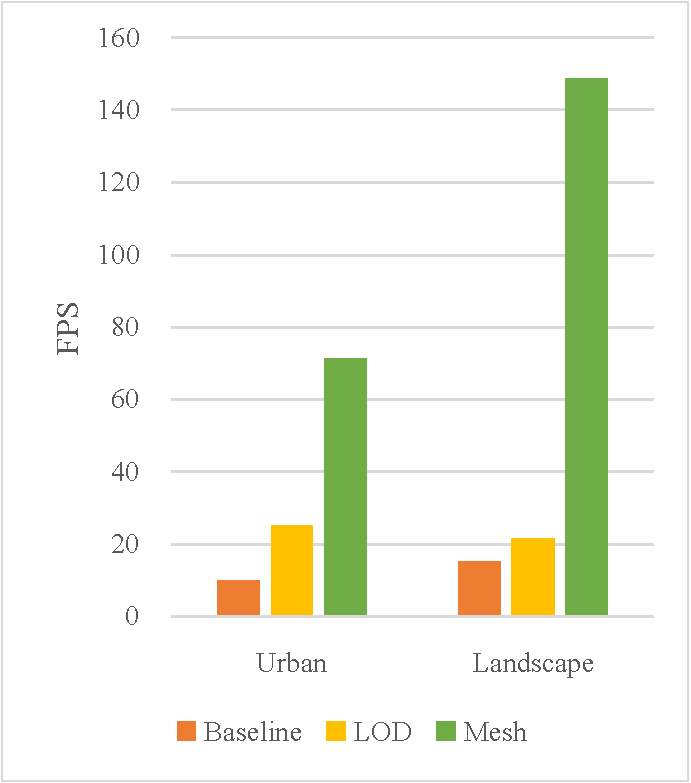
\includegraphics[width=\textwidth]{graph-fps-high.pdf}
        \caption{High quality}
    \end{subfigure}
    %
    \begin{subfigure}{0.3\textwidth}
        \centering
        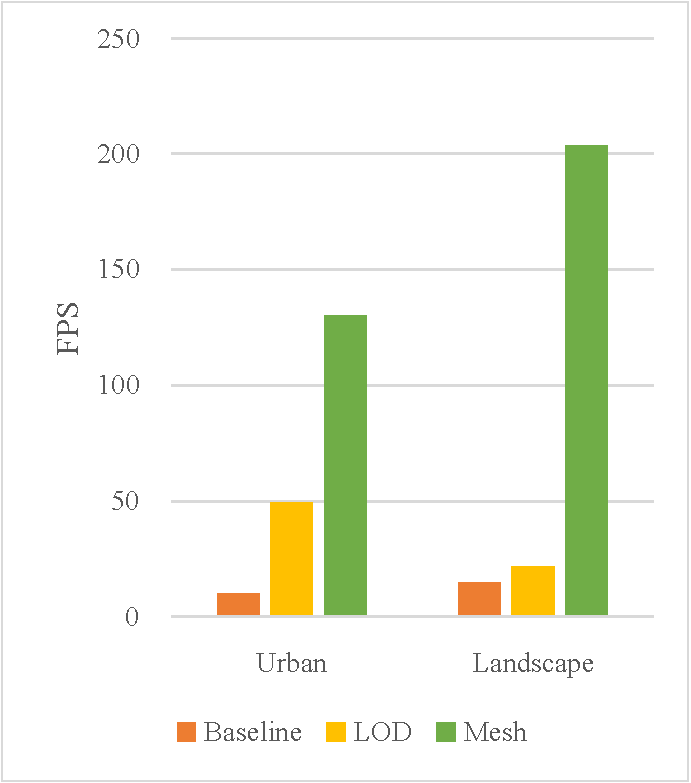
\includegraphics[width=\textwidth]{graph-fps-med.pdf}
        \caption{Medium quality}
    \end{subfigure}
    %
    \begin{subfigure}{0.3\textwidth}
        \centering
        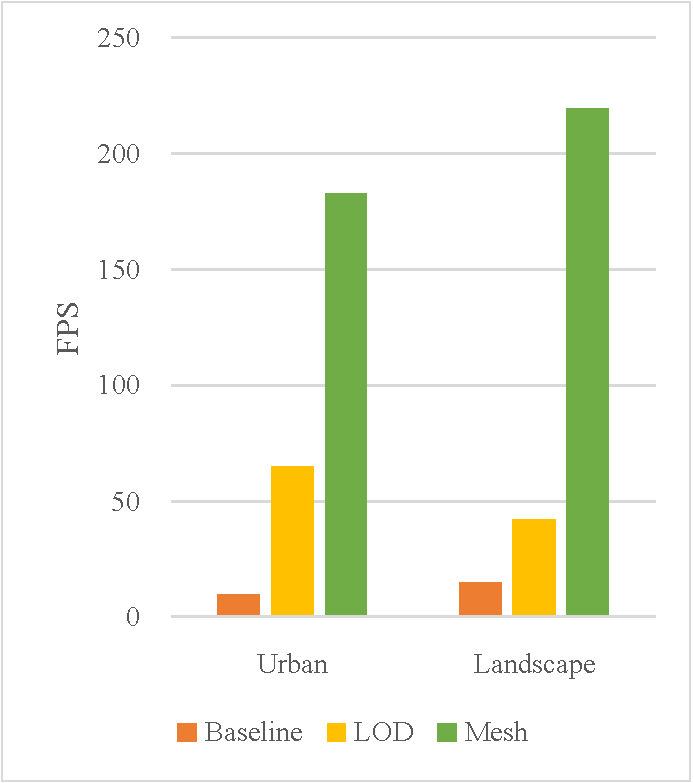
\includegraphics[width=\textwidth]{graph-fps-low.pdf}
        \caption{Low quality}
    \end{subfigure}
    
    \caption{Framerate measured on different quality settings.}
    \label{fig:results:graph-fps}
\end{figure}

The results show that the Mesh generation method demonstrates significant performance improvement over baseline and LOD generation methods.

The LOD generation method shows 2.5x to 6.5x performance improvement compared to baseline on urban scene and 1.1x to 2.8x performance improvement on landscape scene.

The Mesh generation method shows 7.1x to 18.2x performance improvement compared to baseline on urban scene and 9.9x to 14.6x performance improvement on landscape scene.

\subsection{Memory usage}

The \autoref{fig:results:graph-mem} summarizes the results on memory usage.

\begin{figure}[h]
    \centering
    
    \begin{subfigure}{0.3\textwidth}
        \centering
        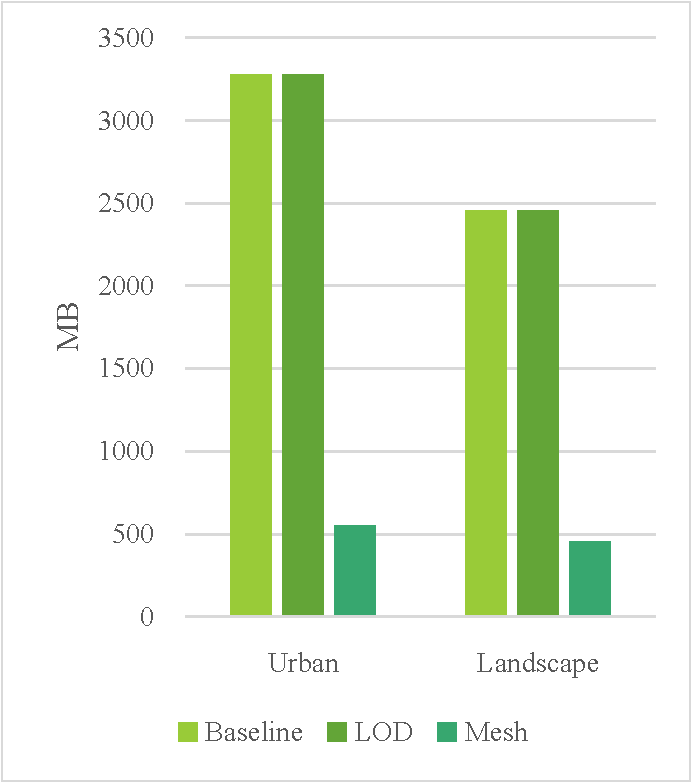
\includegraphics[width=\textwidth]{graph-mem-high.pdf}
        \caption{High quality}
    \end{subfigure}
    %
    \begin{subfigure}{0.3\textwidth}
        \centering
        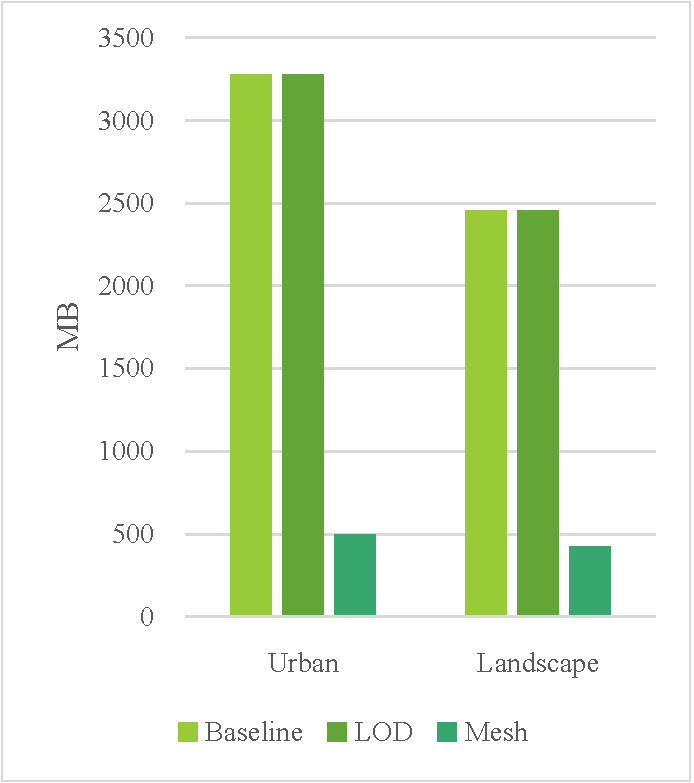
\includegraphics[width=\textwidth]{graph-mem-med.pdf}
        \caption{Medium quality}
    \end{subfigure}
    %
    \begin{subfigure}{0.3\textwidth}
        \centering
        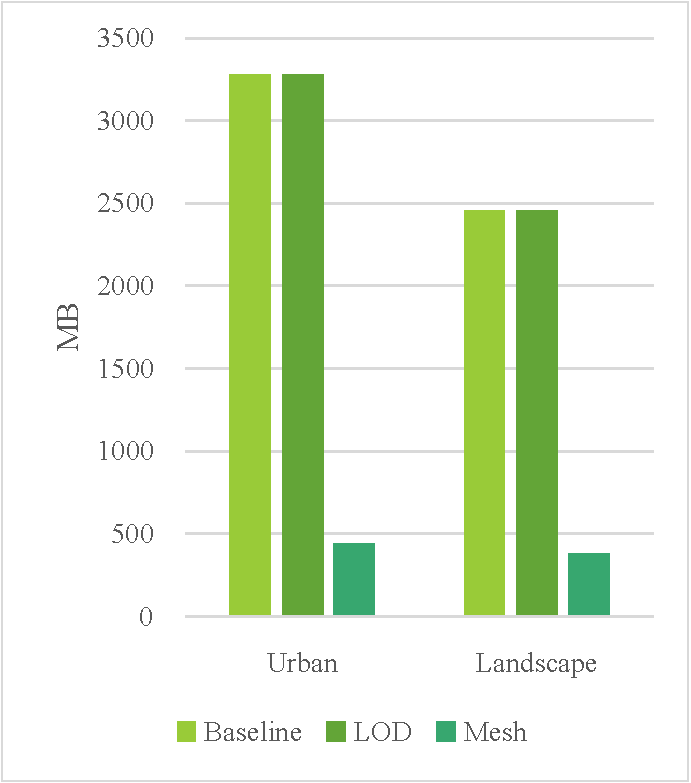
\includegraphics[width=\textwidth]{graph-mem-low.pdf}
        \caption{Low quality}
    \end{subfigure}
    
    \caption{Framerate measured on different quality settings.}
    \label{fig:results:graph-mem}
\end{figure}

The Mesh generation method uses 5.9x to 7.3x times less memory than baseline on urban scene and 5.4x to 6.4x times less memory on landscape scene.

Due to implementation peculiarities, the LOD generation algorithm uses the same amount of memory as the baseline.

\section{Limitations}

\subsection{LOD generation}

The LOD generation algorithm shows good visual quality when observing the scene from a far distance. However, due to the nature of point clouds, it loses detail in a close look. Furthermore, as there is a distance between points, the zoomed point cloud becomes hard to observe.

\begin{figure}[h]
    \centering
    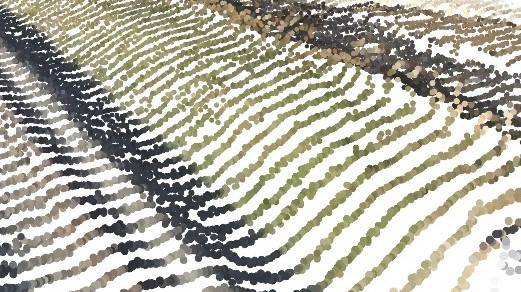
\includegraphics[width=0.7\textwidth]{lod-limitation.jpg}
    \caption{Point cloud visualised with LOD generation algorithm in close look.}
    \label{fig:results:lod-limitation}
\end{figure}

\subsection{Mesh generation}

Although the Mesh generation algorithm demonstrates excellent performance and detail, it has a fundamental flaw: this algorithm cannot correctly handle the scenes with objects placed above the ground, so there is a space between the surface and the object. Examples are bridges, trees, cranes, flying objects. This case is demonstrated on \autoref{fig:results:mesh-edgecase}.

As the algorithm records the highest point of the point cloud, the result will appear as a hill with all the details discarded under it.

\begin{figure}[h]
    \centering
    
    \begin{subfigure}{0.45\textwidth}
        \centering
        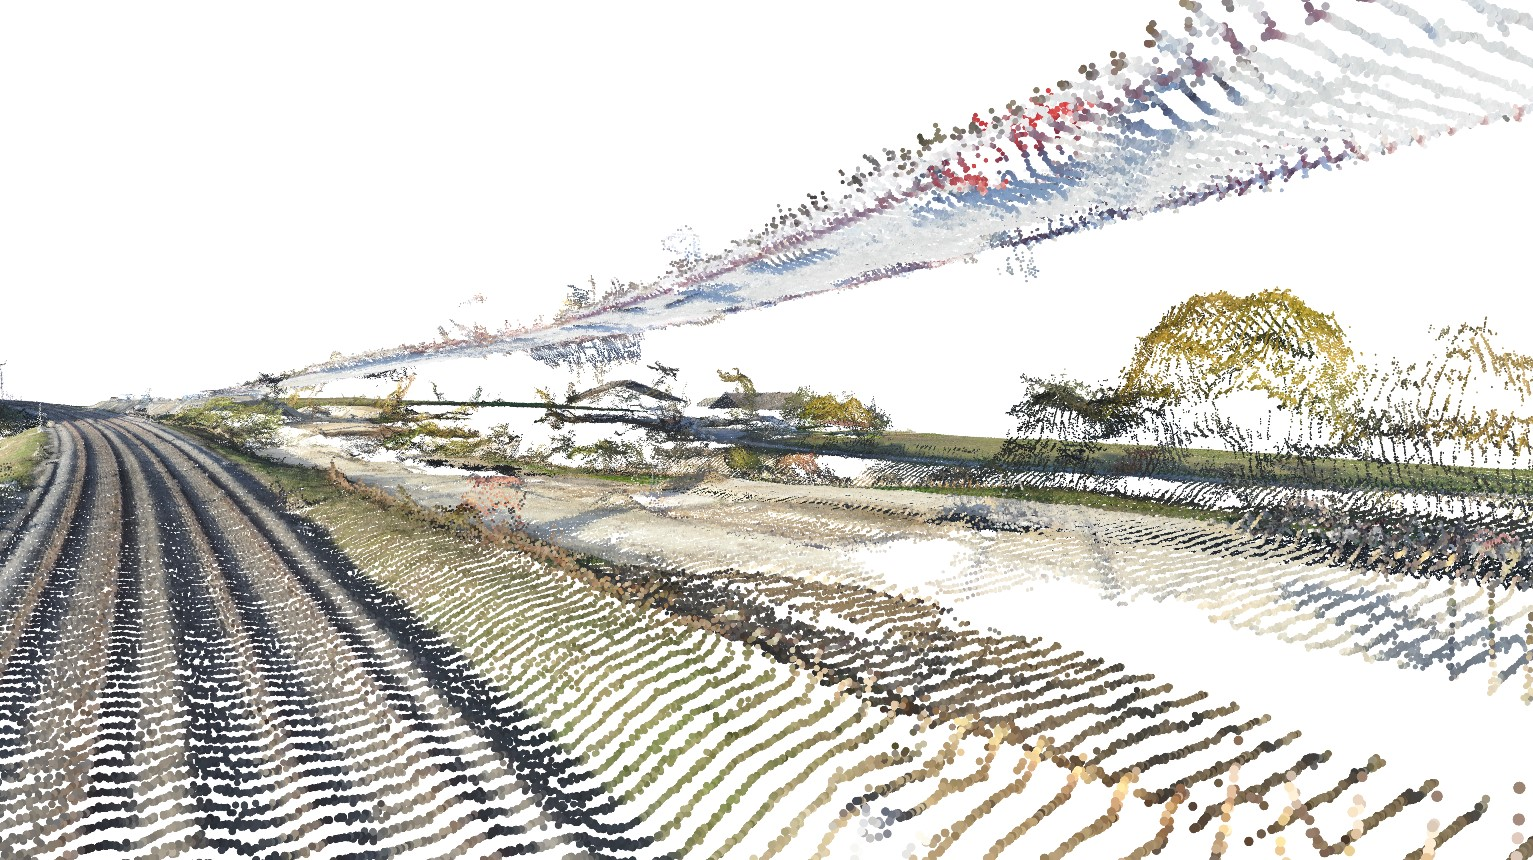
\includegraphics[width=\textwidth]{lod-edgecase.jpg}
        \caption{LOD generation. result}
    \end{subfigure}
    %
    \begin{subfigure}{0.45\textwidth}
        \centering
        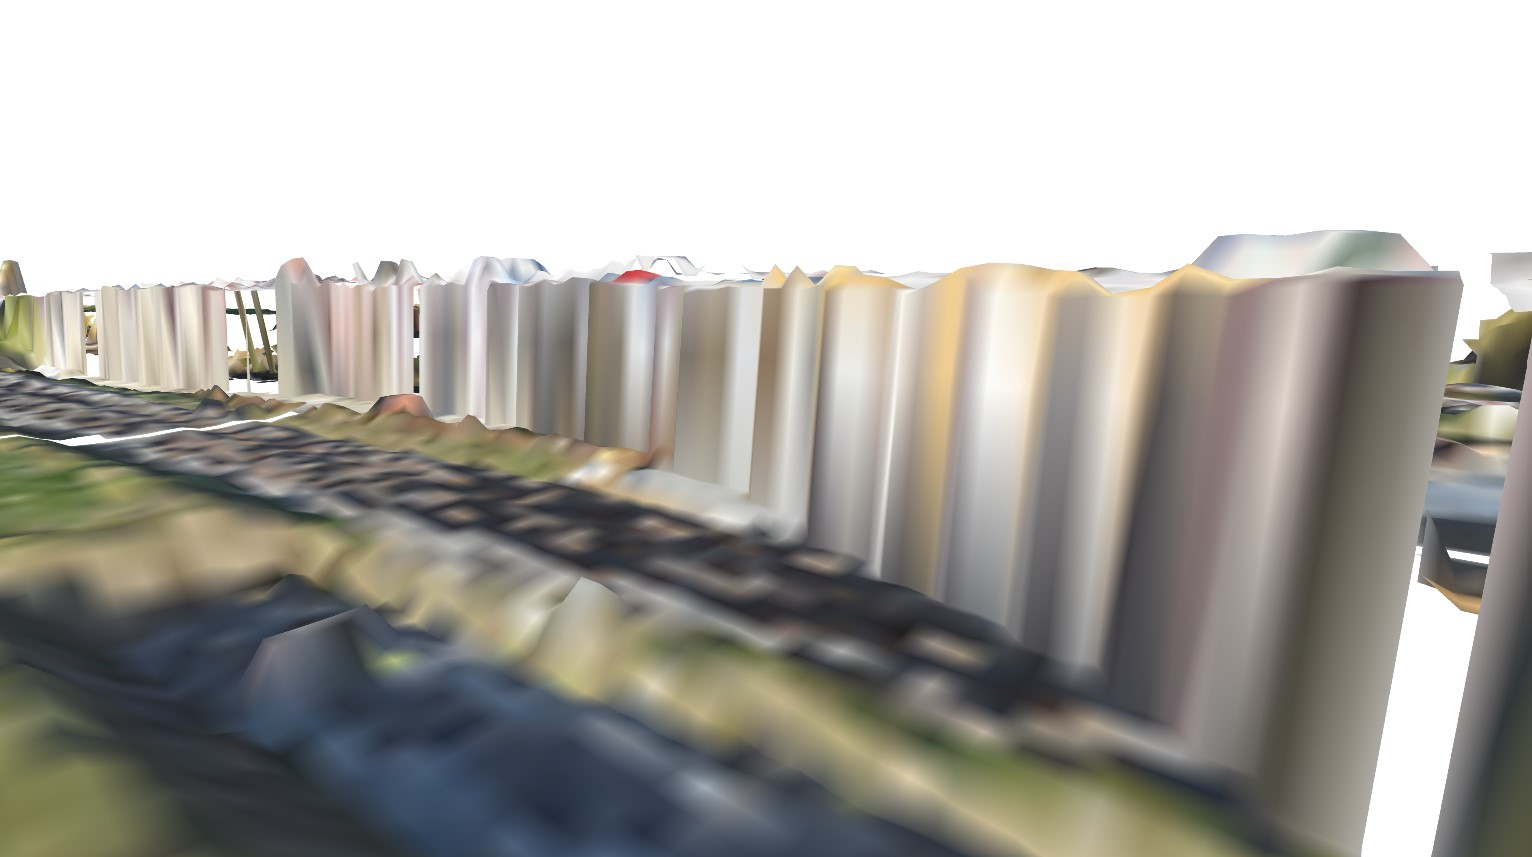
\includegraphics[width=\textwidth]{mesh-edgecase.jpg}
        \caption{Mesh creation result.}
    \end{subfigure}
    
    \caption{An example of edge case for mesh generation algorithm. It discards the detail under the bridge.}
    \label{fig:results:mesh-edgecase}
\end{figure}

Another problem is that the current implementation of the Mesh generation algorithm currently produces noticeable gaps on chunk borders. However, this defect can be eliminated in future work.

\section{Discussion}

It was observed that the Mesh generation method shows a higher performance boost when comparing to the LOD generation method. Mesh generation also uses significantly less memory than LOD generation. However, it has a significant drawback that was discussed above.

The LOD generation algorithm produces good results for observing point clouds from a far perspective. It keeps the detail of the point cloud and correctly handles the complex cases like floating objects that the Mesh generation algorithm might handle erratically. However, it is not applicable for close or precise object examination.

The Mesh generation algorithm should be applicable in most cases. For example, it produces good results when visualizing open landscape areas with simple geometry. Therefore, the Innopolis Simulator team decided to use the Mesh generation in the simulator software.

One might use the LOD generation algorithm for examining the raw point clouds as it visualizes the cloud in its unprocessed form with better performance.

A user should explore the algorithm capabilities and limitations and input data features and choose a suitable algorithm based on these observations.
